\section{Zielsetzung}
\label{sec:Zielsetzung}
Ziel des Versuchs ist die Bestimmung der Wellenlänge eines Lasers und des Brechungsindex von Luft mihilfe eines Michelson-Interferometers.
\section{Theorie}
\label{sec:Theorie}
Das Michelson Interferometer nutzt die Eigenschaft von koheränten Licht, dass es interferiere kann. Koheräntes Licht ist Licht, welches monochromatisch 
und in Phase ist. Für die Intensität $I$ zweier überlagernder Wellen gilt 
\begin{equation}
I = I_1 + I_2 + 2 \sqrt{I_1 \cdot I_2} \cos(\phi_{12})  
\end{equation}
mit $I_1$ als Intensität der 1. Welle, $I_2$ als Intensität der 2. Welle und $\phi_{12}$ als Phasenunterschied. Für deine Intensität einer Welle gilt 
\begin{equation}
    I \propto |E(x,t)|² \, .
\end{equation}
Für Licht gilt die Beziehung $\Delta \nu \cdot \Delta l = c$ mit $\Delta l$ als Länge des Wellenzuges, $\Delta \nu$ als spektrale Bandbreite und $c$ als 
Lichtgeschwindigkeit. Daraus lässt sich schließen, dass nur eine unendlich ausgedehnte Welle monochromatisch sein kann. 
Allerdings lassen sich realistisch auch Koheränzlängen von $1000 \, \unit{\kilo\meter}$ mithilfe eines HeNe - Lasers erzeugen. 
\subsection{Michelson Interferometer}
Das Michelson Interferometer nutzt die Interferenzerscheinungen, um bei bekannter Wellenlänge des Lasers eine Längenänderung oder Brechungsindex 
genau zu bestimmen. Der schematische Aufbau ist in Abbildung (\ref{fig:Aufbau}) zu sehen. 
\begin{figure}[H]
    \centering
    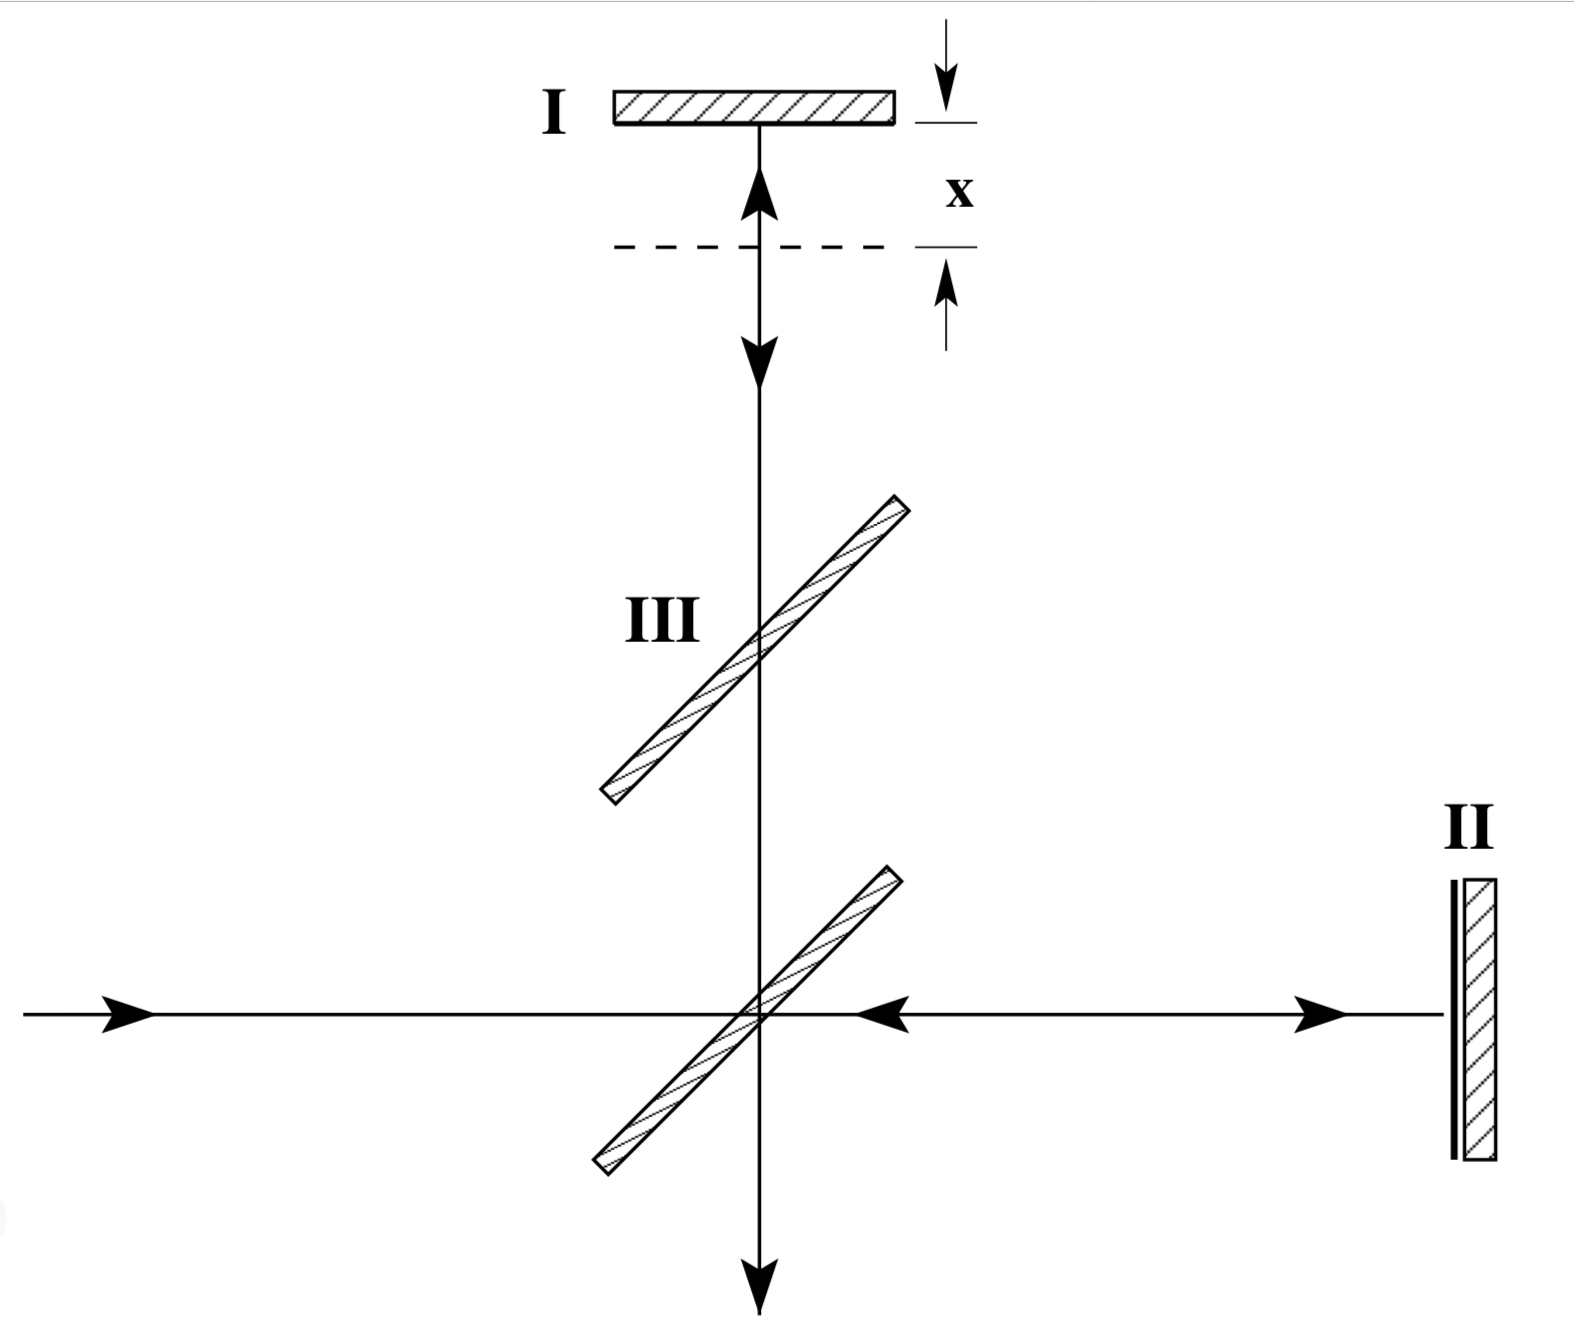
\includegraphics[width=0.6\linewidth]{"content/Bilder/V401.png"}
    \caption{Schematischer Aufbau eines Michelson Interferometer \cite{anleitungV401}.}
    \label{fig:Aufbau}
\end{figure}
Das Michelson Interferometer funktioniert dadurch, dass der eingehende Laserstrahl mithilfe einer Teilerplatte in zwei Strahlen aufgeteilt wird, die sich senkrecht 
zueinander ausbreiten. Der eine Strahl, der am Spiegel reflektiert wird, wird durch eine Glasplatte (III) geleitet, um auszugleichen, dass der andere Teil des Strahls
die Teilerplatte durchdringen musste auf seinem Weg. Dann werden beide Strahlen an einem Spiegel reflektiert. Durch die Teilerplatte werden beide Strahlen wieder 
zusammengeführt, können interferieren und fallen auf einen Schirm. Der Spiegel (I) kann verschoben werden, wodurch sich die Länge, die der Lichtstrahl zurücklegen 
muss verändert. Durch eine Verschiebung um eine halbe Wellenlänge wird ein Interferenzmaximum zu einem Interferenzminumum und umgekehrt. Dadurch kann 
der Abstand $x$ zu 
\begin{equation}
    x = \frac{2}{\lambda \cdot z}
    \label{eqn:x_Formel}
\end{equation}
mit $z$ als Häufigkeit der Wechsels zwischen Minimum und Maximum bestimmt werden. \\
Zur Bestimmung des Brechungsindices von Luft wir die Formel 
\begin{equation}
    D \cdot \Delta n = \frac{z \cdot \lambda}{2}
    \label{eqn:Delta_n_Bestimmen}
\end{equation}
verwendet. $D$ ist dabei die Länge der Gaszelle (in diesem Experiment $50 \,\unit{\milli\meter}$). Mithilfe des idealen Gasgesetzes 
\begin{equation}
    p \cdot V = n \cdot R \cdot T
    \label{eqn:Ideale_Gasgleichung}
\end{equation}
kann die Druckdifferenz $\Delta p$ bestimmt werden. Der Brechungsindex $n$ wird daher durch 
\begin{equation}
    n = 1 + \Delta n \cdot \frac{T}{T_0} \cdot \frac{p_0}{\Delta p}
    \label{eqn:Brechungsindex}
\end{equation}
berechnet. $T_0$ und $p_0$ sind dabei die Temperatur und der Druck bei Normalbedingung. 
\subsection{Vorbereitungsaufgaben}
\label{sec:Vorbereitungsaufgaben}
Zur Vorbereitung sollten die Brechungsindices von Luft, $\ce{CO}$ und $\ce{CO_2}$ recherchiert werden. Der Brechungsindex von Luft ist $1,000292$ \cite{Luft},
 der von $\ce{CO}$ ist $1,0003$ \cite{CO}
und der von $\ce{CO_2}$ ist $1,0004$ \cite{CO_2}. 
